%!TEX root = ../report.tex
\begin{document}
\chapter{Methodology}
In this chapter, we will discuss about RandLA-Net used for 3D semantic segmentation, 
especially about how the RandLA-Net architecture helps in efficient segmentation.
How random point sampling along with local feature aggregation module in RandLA-Net is better than other sampling methods.
We also discuss about the deep ensembles for uncertinty quantification and, we conclude this chapter with the environment and training details for the RandLA-Net with deep ensembles.
\section{RandLA-Net}
As stated in \cite{Hu_2020_CVPR_Randla}, it is a light weight, and efficient neural network architecture for sematic segmentation of 3D point clouds.
From related work section cite here, we can observe that the RandLA-Net architecture is best performing among the point models.
Efficient computation, memory usage and a model with direct application o 3D points are the main motivation when developing the RandLA-Net.
To acheive these goals, RandLA-Net employs random point sampling along with the local feature aggregation module.
Authors in \cite{Hu_2020_CVPR_Randla} proved that by a successive application of random point sampling along with lcoal feature aggregation module effective reduce and extract the features of the large scale point clouds from a scale of $10^5$ to $10^2$.

RandLA-Net utilizes random point sampling among the other sampling methods such as Farthest Point Sampling, Inverse Density Point Sampling.
In random point sampling, we select K points uniformly from original point cloud and has a computational complexity time of O(1).
When compared among other point sampling methods, random point sampling has the lowest computational complexity and computation time is completely independent on number of points.
Despite of these advantages, random point sampling comes with a major disadvantgae of important points being dropped.
To overcome this, authors of RandLA-Net proposed local feature aggragation module for progressive capture of complex features on these selected points.

\begin{figure}
    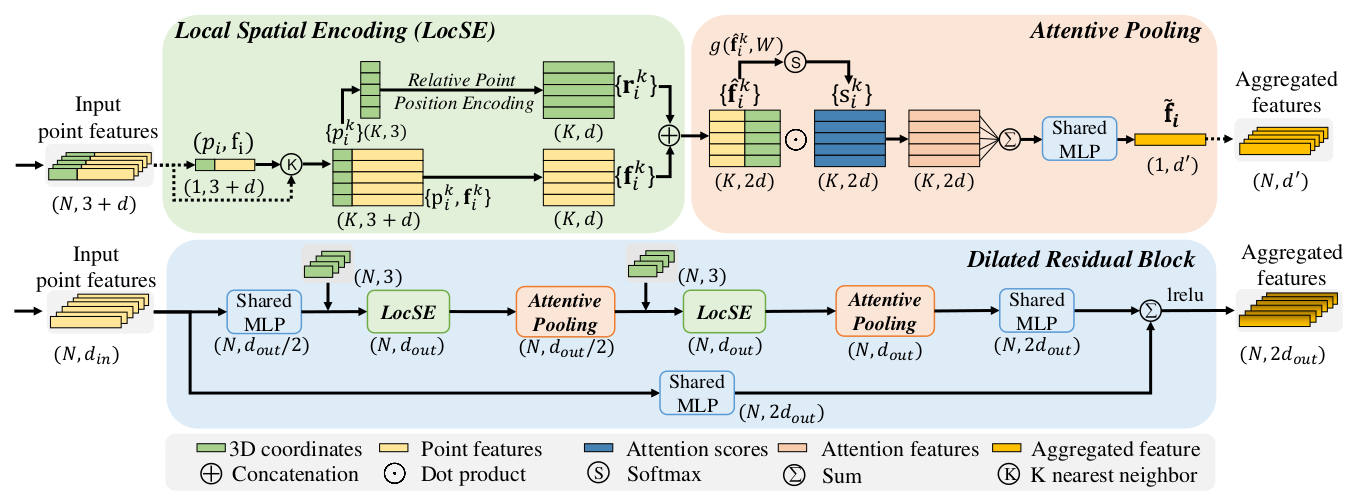
\includegraphics[scale=0.33]{images/localfeatueaggregation-randlanet.png}
    \caption{local feature aggregation module of the randlanet}
    \label{fig:randlanetlfa}
\end{figure}
Figure \ref{fig:randlanetlfa} represents the local features aggregation module for the RandLA-Net.
This module is applied paralleling on the 3D points and architecture of local feature aggregation module is further divided into three sub modules.
They are local spatial encoding (LosSE), attentive pooling and dilated residual block.
Let us discuss further each of these submodules in detail.
\end{document}
